\documentclass[aps,prd,11pt,tightenlines,superscriptaddress,nofootinbib,preprintnumbers,notitlepage]{revtex4-1}

% disable subsections and subsubsections in the TOC
\makeatletter
%\def\l@subsection#1#2{}
\def\l@subsubsection#1#2{}
\makeatother

\pdfoutput=1
\usepackage{amsmath,multirow,graphicx,tabularx,epsfig}
\usepackage{color}
\usepackage{hyperref}


\usepackage{enumerate}
%\newcommand{\ps}[1]{{\color{blue} [Peter] #1}}
%\newcommand{\tp}[1]{{\color{cyan} [Tilman] #1}}
%\newcommand{\fk}[1]{{\color{red} [Felix] #1}}


\def\contentsname{{\normalsize Content}}
\def\tablename{Table}
\def\figurename{Figure}

\def\pveto{P_\text{veto}}
\def\nj{n_\text{jets}}
\def\meff{m_\text{eff}}
\def\ptmin{p_T^\text{min}}
\def\gtot{\Gamma_\text{tot}}
\def\as{\alpha_s}
\def\az{\alpha_0}
\def\gz{g_0}
\def\w{\vec{w}}
\def\sdag{\Sigma^{\dag}}
\def\s{\Sigma}
\newcommand{\psib}{\overline{\psi}}
\newcommand{\Psib}{\overline{\Psi}}
%\newcommand{\dslash}{\not{\hbox{\kern-3pt $\partial$}}}
%\newcommand{\Dslash}{\not{\hbox{\kern-3pt $D$}}}
%\def\one{\leavevmode\hbox{\small1\kern-7.3pt\normalsize1}}
%%\def\one{I}
\newcommand\one{\leavevmode\hbox{\small1\normalsize\kern-.33em1}}
\newcommand{\Mpl}{M_\mathrm{Pl}}
%\def\dslash{\not{\hbox{\kern-4pt $\partial$}}}
%\def\Dslash{\not{\hbox{\kern-4pt $D$}}}
\newcommand{\p}{\partial}
\newcommand{\mat}{\mathcal{M}}
\newcommand{\lag}{\mathcal{L}}
\newcommand{\ord}{\mathcal{O}}
\newcommand{\ope}{\mathcal{O}}
\newcommand{\qqquad}{\qquad \qquad}
\newcommand{\qqqquad}{\qquad \qquad \qquad}
 
\newcommand{\ds}{\displaystyle}
\newcommand{\qb}{\bar{q}}
\newcommand{\matx}{|\mathcal{M}|^2}
%\newcommand{\mat}{\mathcal{M}}
%\newcommand{\slashed}[1]{\ensuremath{{#1}{\!}{\!}{\!}{\!}{\:}/}}
\newcommand{\really}{\stackrel{!}{=}}
\newcommand{\msbar}{\overline{\text{MS}}}
\newcommand{\qns}{f_q^\text{NS}}
\newcommand{\lqcd}{\Lambda_\text{QCD}}
\newcommand{\met}{\slashchar{p}_T}
\newcommand{\pmiss}{\slashchar{\vec{p}}_T}

\newcommand{\sq}{\tilde{q}}
\newcommand{\go}{\tilde{g}}
\newcommand{\st}[1]{\tilde{t}_{#1}}
\newcommand{\stb}[1]{\tilde{t}_{#1}^*}
\newcommand{\nz}[1]{\tilde{\chi}_{#1}^0}
\newcommand{\cp}[1]{\tilde{\chi}_{#1}^+}
\newcommand{\cm}[1]{\tilde{\chi}_{#1}^-}
\newcommand{\CP}{CP}

% all the masses 
\providecommand{\mg}{m_{\tilde{g}}}
\providecommand{\mst}[1]{m_{\tilde{t}_{#1}}}
\newcommand{\msn}[1]{m_{\tilde{\nu}_{#1}}}
\newcommand{\mch}[1]{m_{\tilde{\chi}^+_{#1}}}
\newcommand{\mne}[1]{m_{\tilde{\chi}^0_{#1}}}
\newcommand{\msb}[1]{m_{\tilde{b}_{#1}}}
\newcommand{\vsm}{\ensuremath{v_\text{SM}}}

% units of measure
\newcommand{\mev}{\text{MeV}}
\newcommand{\gev}{\text{GeV}}
\newcommand{\tev}{\text{TeV}}
\newcommand{\fb}{\text{fb}}
\newcommand{\ab}{\text{ab}}
\newcommand{\pb}{\text{pb}}
\newcommand{\br}{\text{BR}}
\newcommand{\sign}{\text{sign}}
\newcommand{\iab}{\text{ab}^{-1}}
\newcommand{\ifb}{\text{fb}^{-1}}
\newcommand{\ipb}{\text{pb}^{-1}}
\newcommand{\itevx}{\text{TeV}^{-2}}

% really great macro by Chris Lester
\def\slashchar#1{\setbox0=\hbox{$#1$}           % set a box for #1
   \dimen0=\wd0                                 % and get its size
   \setbox1=\hbox{/} \dimen1=\wd1               % get size of /
   \ifdim\dimen0>\dimen1                        % #1 is bigger
      \rlap{\hbox to \dimen0{\hfil/\hfil}}      % so center / in box
      #1                                        % and print #1
   \else                                        % / is bigger
      \rlap{\hbox to \dimen1{\hfil$#1$\hfil}}   % so center #1
      /                                         % and print /
   \fi}
\newcommand{\dslash}{\slashchar{\partial}}
\newcommand{\Dslash}{\slashchar{D}}

\newcommand{\eg}{\textsl{e.g.}\;}
\newcommand{\ie}{\textsl{i.e.}\;}
\newcommand{\Ie}{\textsl{I.e.}\;}
\newcommand{\etal}{\textsl{et al}\;}
\DeclareMathOperator{\tr}{Tr}

% maximal number of floating environments on each page 
\setlength{\floatsep}{0pt}
\setcounter{topnumber}{1}
\setcounter{bottomnumber}{1}
\setcounter{totalnumber}{1}
\renewcommand{\topfraction}{1.0}
\renewcommand{\bottomfraction}{1.0}
\renewcommand{\textfraction}{0.0}
\renewcommand{\thefootnote}{\fnsymbol{footnote}}

\newcommand{\rig}{\rightarrow}
\newcommand{\lrig}{\longrightarrow}
\renewcommand{\d}{{\mathrm{d}}}
\newcommand{\be}{\begin{eqnarray*}}
\newcommand{\ee}{\end{eqnarray*}}
\newcommand{\gl}[1]{(\ref{#1})}
\newcommand{\ta}[2]{ \frac{ {\mathrm{d}} #1 } {{\mathrm{d}} #2}}
\newcommand{\bee}{\begin{eqnarray}}
\newcommand{\eee}{\end{eqnarray}}
\newcommand{\beeq}{\begin{equation}}
\newcommand{\eeeq}{\end{equation}}
\newcommand{\mc}{\mathcal}
\newcommand{\mr}{\mathrm}
\newcommand{\ep}{\varepsilon}
\newcommand{\eps}{\varepsilon}
%\renewcommand{\vec}{\bf}
\newcommand{\emt}{$\times 10^{-3}$}
\newcommand{\emfo}{$\times 10^{-4}$}
\newcommand{\emfi}{$\times 10^{-5}$}

\newcommand{\revision}[1]{{\bf{}#1}}

\newcommand{\hzero}{h^0}
\newcommand{\Hzero}{H^0}
\newcommand{\Azero}{A^0}
\newcommand{\PHiggs}{H}
\newcommand{\PW}{W}
\newcommand{\PZ}{Z}

\newcommand{\sw}{\ensuremath{s_w}}
\newcommand{\cw}{\ensuremath{c_w}}
\newcommand{\swd}{\ensuremath{s^2_w}}
\newcommand{\cwd}{\ensuremath{c^2_w}}
%
%% 2HDM Higgs masses
\newcommand{\mhhd}{\ensuremath{m^2_{\Hzero}}}
\newcommand{\mhh}{\ensuremath{m_{\Hzero}}}
\newcommand{\mlhd}{\ensuremath{m^2_{\hzero}}}
\newcommand{\Mlh}{\ensuremath{m_{\hzero}}}
\newcommand{\mad}{\ensuremath{m^2_{\Azero}}}
% \newcommand{\ma}{\ensuremath{m_{\Azero}}}
\newcommand{\mhpd}{\ensuremath{m^2_{\PHiggs^{\pm}}}}
\newcommand{\mhp}{\ensuremath{m_{\PHiggs^{\pm}}}}

%% GPS: the following defs have been commented out
%%      because one of them interfered with the \url package
%\newcommand{\sa}{\ensuremath{\sin\alpha}}
%\newcommand{\ca}{\ensuremath{\cos\alpha}}
%\newcommand{\cad}{\ensuremath{\cos^2\alpha}}
%\newcommand{\sad}{\ensuremath{\sin^2\alpha}}
%\newcommand{\sbd}{\ensuremath{\sin^2\beta}}
%\newcommand{\cbd}{\ensuremath{\cos^2\beta}}
%\newcommand{\cb}{\ensuremath{\cos\beta}}
%\renewcommand{\sb}{\ensuremath{\sin\beta}}
%\newcommand{\tanbd}{\ensuremath{\tan^2\beta}}
%\newcommand{\cotbd}{\ensuremath{\cot^2\beta}}
%\newcommand{\tanb}{\ensuremath{\tan\beta}}
%\newcommand{\tb}{\ensuremath{\tan\beta}}
%\newcommand{\cotb}{\ensuremath{\cot\beta}}


% trying to make it look okay for A4 and for letter formats
%\addtolength{\topmargin}{10mm}
\addtolength{\evensidemargin}{-5mm}
\addtolength{\oddsidemargin}{-5mm}
%\addtolength{\textheight}{5mm}
\addtolength{\textwidth}{10mm}

\newcommand{\hepstore}{\texttt{HepStore}}
\newcommand{\python}{\texttt{Python~2.7}}
\newcommand{\docker}{\texttt{Docker}}


\usepackage{framed}
\usepackage{listings}
\usepackage{color}

\definecolor{dkgreen}{rgb}{0,0.6,0}
\definecolor{gray}{rgb}{0.5,0.5,0.5}
\definecolor{mauve}{rgb}{0.58,0,0.82}

\usepackage{inconsolata}

\definecolor{aqua}{rgb}{0.0, 1.0, 1.0}
\definecolor{babyblue}{rgb}{0.54, 0.81, 0.94}


\lstdefinelanguage{Python2}{%
  language     = Python,
  morekeywords = {self},
}


\lstset{frame=tb,
  language=Python2,
  aboveskip=3mm,
  belowskip=3mm,
  showstringspaces=false,
  columns=flexible,
  basicstyle={\small\ttfamily},
  numbers=none,
  numberstyle=\tiny\color{gray},
  keywordstyle=\color{blue},
  commentstyle=\color{dkgreen},
  stringstyle=\color{mauve},
  breaklines=true,
  breakatwhitespace=true,
  keepspaces=true
  tabsize=3,
  emph={ True, False, None},
  emphstyle={ \color{babyblue}}
}

\def\changemargin#1#2{\list{}{\rightmargin#2\leftmargin#1}\item[]}
\let\endchangemargin=\endlist 

%%%%%%%%%%%%%%%%%%%%%%%%%%%%%%%%%%%%%%%%%%%%%%%%%%%%%%%%%%%%%%%%%%%%%%%%
\begin{document}
\title{{\bf\Huge\hepstore: The Awakening}}

\preprint{IPPP/16/72}

\author{Peter Schichtel}
\affiliation{Institute for Particle Physics Phenomenology, Durham University, UK}
\email{peter.schichtel@durham.ac.uk}


\begin{abstract}
  A framework to trade (hence the name) your phenomelogy analysis in a preserved way. 
\end{abstract}

\maketitle

\bigskip 
\bigskip 

\tableofcontents 

\newpage

%%%%%%%%%%%%%%%%%%%%%%%%%%%%%%%%%%%%%%%%%%%%%%%%%%%%%%%%%%%%%%%%%%%%%%%%

\section{Installation}
\label{sec:installation}

The \hepstore~--~Framework is written solely in \python. To install
the package you need 'pip'~\cite{}.
%
\begin{framed}
  \begin{center}
    pip install (-{}-upgrade) (-{}-user) git+https://github.com/PeterSchichtel/hepstore.git
  \end{center}
\end{framed}
%
The arguments in parenthesis are optional. Furthermore, if you want to
make use of the {\bf Monte~Carlo reproducability features} in
\hepstore~you need a working Docker~\cite{} installation.

\section{The \hepstore~--~Framework}
\label{sec:framework}

In the following we will outly the core modules hepstore is composed
of. We will introduce their usage and motivation and give examples of
their simple usability.

\subsection{hepstore.docker:~~~Monte Carlo Reproducibility}

\subsubsection{Reproducibility}

Reproducing any result from previous scientific work is at the heart
of the scientific method. It occures often that ground breaking
scientific results are doubted for many years until reproduced
correctly. Contrary, if not reproduced at all, the result is simply
not believed to be true~\cite{}. It is therefore obvious and vital to
any scientific effort to be easily reproduced. Of course, for some
experimental setup this just might not be easily done. It might be
that the experience needed to craft a certain item just has been
developed during the actual research itself. However, in the high
energy physics community, more and more scientific results completely
depend on work performed by computers. And indeed, there has been
tremondous effort in the experimantal LHC community to achive high
scientific standards of reproducibility. Namely the
\texttt{REANA}~\cite{} frame work.

However, one should not think that no such efforts have been
undertaken in the phenomelogical community. There is
\texttt{MadAnalysis5}~\cite{} which has the ability to recast LHC
analyses and provides a convienent frame work for high energy physics
analyses. There is, of course, \texttt{Rivet}~\cite{}, which comes
along with \emph{actual, verified} phenomenolgical and experimental
analyses. There is the \texttt{ROOT}~\cite{} framework which provides
a multitude of analysis tools. These tools provide building blocks to
perform, save and eventually redo any analysis. In addition, the Monte
Carlo (MC) code developers~\cite{} provide ever simpler installation
routines for their code packages, including interfaces to third party
software.

So, why bother with the reproducibility of phenomenoligical results?
It is true that a fair amount of the analysis itself is either
automated or can be easily build from freely availbale
software. However, that does not mean that it is actually
reproducible. Anybody who has ever tried to redo what they or someone
else did five years ago might already know some of the problems:
library missing, code missing, data missing, does not compile anymore,
does not run anymore, 32-bit what?, not supported, what was the random
seed again, which version of package XY was used, etc. pp.

%
\begin{minipage}{\textwidth}
  Let us start with defining the neccessary conditions for a
  phenomenolgical analysis to be \emph{fully reproducible}.
  %
  \begin{enumerate}[(a)]
  \item The state of the machine can be {\bf frozen} and published.
  \item Except for the state of the machine, the work only depends on
    simple (i.e text), publishable {\bf input files}.
  \item The full analysis chain can be invoked by means of a
    {\bf platform independent} command.
  \end{enumerate}
  %
\end{minipage}
\medskip
%

Requirement (a) is most easily solved by invoking
\docker~\cite{}. \docker~is a framework which allows to ship
containerized applications. This means it is able to produce a frozen
state of a machine. The \docker~image contains all the libraries and
packages installed during its creation. Furthermore, \docker~hosts a
webpage where one can upload and therefore publish \docker~images.

Requirement (b) is most of the time already satisfied by todays
publications, where run and parameter cards are added as supplimental
material.

Requirement (c) is more tricky, though. Furthermore, it needs
motivation as its neccassity is not as straight forward as (a) and
(b). Note, that the aim of the above description is the full
reproduction of a phenomenoligical analysis. This includes not only
the state of the machine and any input parameters, but also what
commands to run in which order to perform the full analysis. This also
includes any code written specifically for this analysis. Furthermore,
we require platform independence. Who ever replicates the analysis
should not fail due to any special platform requirements. This is
where hepstore.docker enters the stage. It provides a simple
\python~interface to run any command on a given docker image. We show
the source code in the following:
%
\begin{changemargin}{1.5cm}{1.5cm} 
  \lstinputlisting[numbers=left,firstnumber=8,firstline=8]{../../hepstore/docker/interface.py}
\end{changemargin}
%
As a starting point using this interface we provide simple command
line tools for
%
\begin{itemize}
\item Herwig 7.0 ~$~~\rightarrow$ 'hepstore-herwig',
\item Sherpa 2.2 ~$~~\rightarrow$ 'hepstore-sherpa',
\item Corsika 7.4 $~~\rightarrow$ 'hepstore-corsika',
\end{itemize}
%
in accordance with the points raised above: frozen state and platform
independent. The actual code and the docker files can be found in
App.~\ref{app:docker}. Note, however, that Sherpa actually has an
official docker account, where we pull their image from. It is also
the aim of this work to motivate further official docker images from
code developers.

Furthermore, let us provide an example showing the simplicity and
elegance of hepstore.docker. Provided the runcard 'ExampleRunCard.in'
also found in App.~\ref{app:docker}, the following lines og code will
always produce the very same result on any machine:
%
\begin{changemargin}{1.5cm}{1.5cm} 
  \begin{lstlisting}[language=Bash]
    #!/usr/bin/env bash
    hepstore-herwig read ExampleRunCard.in
    hepstore-herwig run  ExampleRunCard.run -N 1000 -s 687\end{lstlisting}
\end{changemargin}
%
Not only have we provided a completely reproducible MC run, there is
also no installation of additional code then \hepstore~neccessary.

\subsection{hepstore.plot:~~~~~~\,Simple Plotting}

In the case where you are not able to use the rivet or madanalysis
plotting capabilities, \hepstore provides a simple user interface
'hepstore-plot' which can plot any one or two dimensional
representation of your data\footnote{provided in .npy
  format}. Currently the following kinds of plots are suported:
scatter, histogram, errorbar, line, errorband, and contour.

\subsubsection{Data Format}

\hepstore~uses the '.npy' format

\subsubsection{Example}
produce some data
%
\begin{changemargin}{1.5cm}{1.5cm} 
  \lstinputlisting[numbers=left,firstnumber=1,firstline=1]{../examples/hepstore_plot/produce_data.py}
\end{changemargin}
%
plot with hepstore-plot
%
\begin{changemargin}{1.5cm}{1.5cm} 
  \lstinputlisting[numbers=left,firstnumber=1,firstline=1,language=Bash]{../examples/hepstore_plot/example.sh}
\end{changemargin}
%
%
show plots
%
\begin{figure}
  \centering
  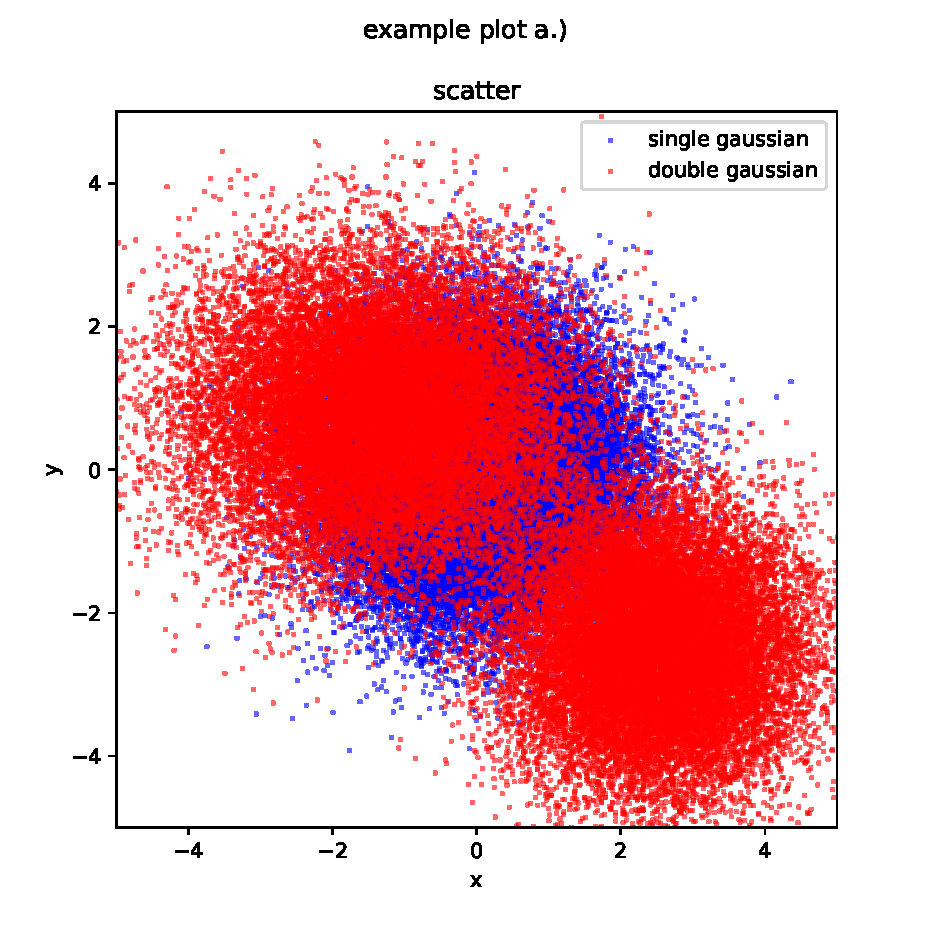
\includegraphics[width=0.3\textwidth]{../examples/hepstore_plot/example_a.pdf}
  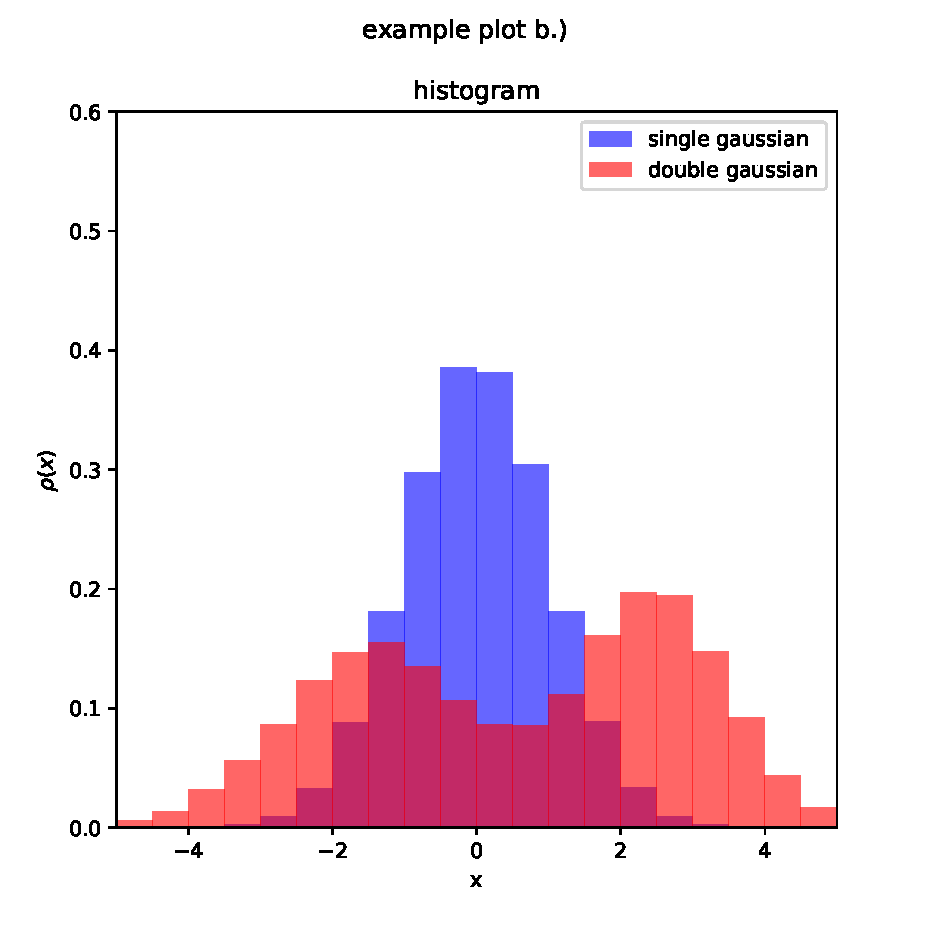
\includegraphics[width=0.3\textwidth]{../examples/hepstore_plot/example_b.pdf}
  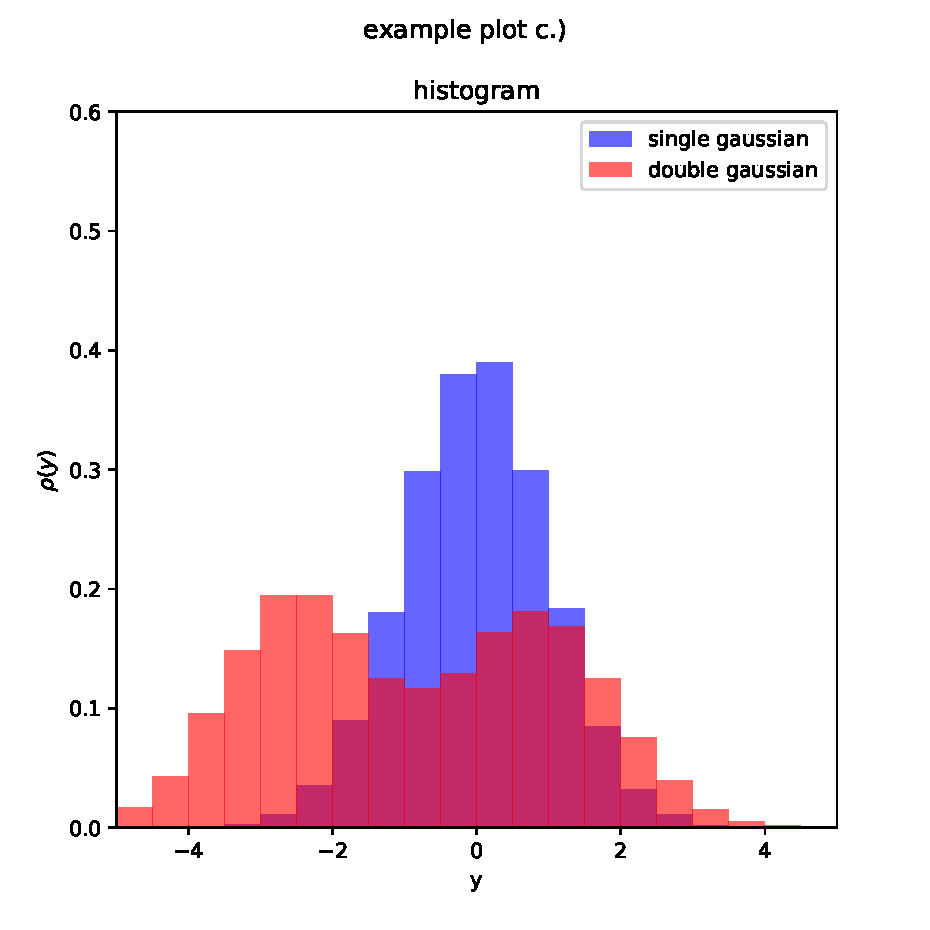
\includegraphics[width=0.3\textwidth]{../examples/hepstore_plot/example_c.pdf}
  \caption{}
  \label{fig:example_plotting}
\end{figure}
%


\subsection{hepstore.school:~~~\,Machine Learning}

One of the themes very interesting to particle physiscts and also
recieving more and more attention in the phenomenolgical community is
machine learning. 'hepstore.school' is an attempt to provide a genric
interface to python's sklearn package. our school consists of a
teacher, a student and, of course, a book. the teacher advices the
student which algorithm to use, where upon the student takes the
algorithm from the book and is able to explore and train itself to
learn from the data provided.

\subsubsection{Classifiers}

lda,qcd,svc,mlp

\subsubsection{Tuning}

As it is not a prior clear which parameters to chose for an algorithm,
'hepstore-school' provides the switch '-{}-only\_explore' which will
try to automatically find the best parameters for the given training
set. In addition for all numerical parameters it provides cross
validation plots to check for over respectively under
performance. Note that some classifiers might have a large parameter
space and hence can not be tunde in a fully automated way, yet.

\subsubsection{Training}

Training is performed automattically on a $75\%$ subset of the data provided.

\subsubsection{Testing}

Training is performed automattically on a $25\%$ subset of the data provided.

\subsubsection{Example}

same data as above

%
%
%
\begin{changemargin}{1.5cm}{1.5cm} 
  \lstinputlisting[numbers=left,firstnumber=1,firstline=1,language=Bash]{../examples/hepstore_school/example.sh}
\end{changemargin}
%
show plots
%
\begin{figure}
  \centering
  \includegraphics[width=0.22\textwidth]{../examples/hepstore_school/tol.pdf}
  \includegraphics[width=0.22\textwidth]{../examples/hepstore_school/reg_param.pdf}
  \includegraphics[width=0.22\textwidth]{../examples/hepstore_school/roc.pdf}
  \includegraphics[width=0.22\textwidth]{../examples/hepstore_school/probability_map.pdf}
  \caption{}
  \label{fig:example_plotting}
\end{figure}
%


\subsection{hepstore.analysis: Automated Hep Analysis}

the hepstore-analysis module is a high level package to perform the
usual statistical computations needed in high energy physics. it
utilizes hepstore.school to provide signal and background
classification and extract statistical quantities such as the maximal
poissonian significance, the upper exclusion bound on the signal cross
section etc.

still missing: traditional cut analysis

\subsubsection{Example}

\section{Produce and Anlyse Extended Air Showers the \hepstore~way: hepstore-eas}

\subsection{List}
'hepstore-eas -L'

As this is a specific air shower framework we organise everything with
respect to the following scheme: energy -> primary particle ->
physical process -> MC generator -> nucleon model -> final state the
-{}-list argument searches for this structure and lists the following
possible contents hard events -> attempted showers -> showeres ->
observables

\subsection{Generation}

'hepstore-eas -G'

we interface from the hepstore.docker family (more details in
appendix) and provide automated runcards for herwig to produce events
which may be showerd by corsika

\subsubsection{Nucleon Modle}

we provide two nucleon models 'full' and 'fragmented'

\subsection{Shower}

'hepstore-eas -S'

we interface from the hepstore.docker family and provide automated
runcards for corsika to either shower events generted with '-G' or
produce corsika stand alone showers (internal corsika di-jet
production) when using '-C 7.4' (here 7.4 is the version vor the
docker image)

\subsection{Observables}

'hepstore-eas -A'

we provide our own event class to read corsika produced extended air
showers. inspired by rivet we allow for dynamic load of user analysis
modules and provide one example for such, constructing $\rho_\mu$ and
$X_\text{max}$. hepstore-eas automatically provides its output in .npy
format

\subsection{Example}

\subsubsection{A User Analysis}

\subsubsection{Comparing Herwig 7 di-jet production with internal Corsika QCD model}

\section{Contributions and Requests}

\section{Conclusions}

\begin{appendix}

  \section{The hepstore.docker family}
  \label{app:docker}

  \subsection{hepstore-herwig}

  \subsubsection{Code}
  %
  \begin{changemargin}{1.5cm}{1.5cm} 
    \lstinputlisting[numbers=left,firstnumber=1,firstline=1]{../../hepstore/docker/herwig.py}
  \end{changemargin}
  %

  \subsubsection{Dockerfile}
  %
  \begin{changemargin}{1.5cm}{1.5cm} 
    \lstinputlisting[numbers=left,firstnumber=1,firstline=1,language=Bash]{../../../../Herwig/HerwigDocker/7.0.4/Dockerfile}
  \end{changemargin}
  %

  \subsubsection{Example Runcard}
  %
  \begin{changemargin}{1.5cm}{1.5cm} 
    \lstinputlisting[numbers=left,firstnumber=1,firstline=1,language=Bash]{../examples/hepstore_docker/ExampleRunCard.in}
  \end{changemargin}
  %
  
  \subsection{hepstore-corsika}

  \subsubsection{Code}

  \subsubsection{Dockerfile}
  
  \subsection{hepstore-hepmc2corsika}

  \subsubsection{Code}

  \subsubsection{Dockerfile}

\end{appendix}


\end{document}
 
 
 

 
 




